\documentclass{standalone}

\usepackage{tikz}
\usepackage{circuitikz}

\tikzset{block/.style = {draw, fill=white, very thick, rectangle, minimum height=1cm, minimum width=2cm},
         lblock/.style={draw,fill=white,very thick, rectangle, minimum height=3cm, minimum width=1cm},
         sum/.style= {draw, fill=white, very thick, circle, node distance=0.5cm}}

         
\begin{document}
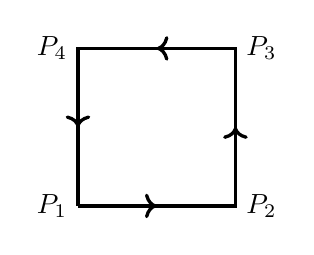
\begin{tikzpicture}[scale=2]
    \draw[-, very thick](0,0)node[left]{$P_1$}--(1,0)node[right]{$P_2$}--(1,1)node[right]{$P_3$}--(0,1)node[left]{$P_4$}--(0,0);
    \draw[->,very thick](0,0)--(0.5,0);
    \draw[->,very thick](1,0)--(1,0.5);
    \draw[->,very thick](1,1)--(0.5,1);
    \draw[->,very thick](0,1)--(0,0.5);
\end{tikzpicture}
\end{document}